\documentclass[a4paper, 12pt]{article}
\usepackage[T1]{fontenc}
\usepackage{lmodern}
\usepackage{color}
\usepackage{amsfonts}
\usepackage{epstopdf}
\usepackage{matlab}
%\documentclass{book}
\usepackage{blindtext}
\usepackage{hyperref}
\usepackage[brazil]{babel}
\usepackage{amssymb}
\usepackage[utf8]{inputenc}
\usepackage{amsmath}
\usepackage{indentfirst}
\usepackage{graphicx}
\usepackage{multicol,lipsum}
\usepackage[a4paper,
top=3cm, left=3cm, bottom=3cm, right=3cm]{geometry}
\usepackage{setspace}
\usepackage{multirow}
\usepackage{float}
\usepackage[dvipsnames]{xcolor}
\usepackage[table]{xcolor}
%\usepackage{pdflscape}
\usepackage[DIV=15]{typearea}
\usepackage[nottoc]{tocbibind}
\usepackage[sort,numbers]{natbib}
%\usepackage{cite}
\usepackage{matlab}

\usepackage[utf8]{inputenc}
\usepackage[T1]{fontenc}
\usepackage{lmodern}
\usepackage{graphicx}
\usepackage{color}
\usepackage{hyperref}
\usepackage{amsmath}
\usepackage{amsfonts}
\usepackage{epstopdf}
\usepackage[table]{xcolor}
\usepackage{matlab}


\documentclass[letterpaper]{article}
% bib pack %%%%%%%%%%%%%%%%%%%%%%%%%%%%%%%%%%%%%%%%%%%%%%%%%%%%%%%%%%%%%%%%%%%%%
\usepackage[utf8]{inputenc}
\usepackage{geometry}
    \geometry{left=3cm,right=2cm,top=2cm,bottom=2cm}
%
\usepackage[spanish]{babel}
%
\usepackage[fixlanguage]{babelbib}
    \bibliographystyle{babunsrt}
%
\usepackage{url}

\begin{document}
%\maketitle

\begin{titlepage}
	\begin{center}
		

\vspace{10pt}
%\begin{figure}[H][!ht]
%\centering
%
\includegraphics{puc-rio-logo.png}

%\end{figure}
\begin{figure}[!ht]
\centering

\includegraphics{images/puc-rio-logo.png}
\end{figure}
\huge{Dinâmica de Sistemas}
        \vspace{70pt}
        
		\textbf{ENG1730}
		\textbf{\large{\\ }}
		
		\vspace{30pt}
		\textbf{\small{\\Lista 07}}
		\vspace{75pt}
		
	\end{center}
	
	\begin{flushleft}
		\begin{tabbing}
			Aluno(a)\qquad\qquad\=\>Paloma Fernanda Loureiro Sette - 1621595\\
			
			Professor(a)\>João Carlos Virgolino Soares\\
	\end{tabbing}
		  
	\end{flushleft}
	\begin{center}
		%\vspace{\fill}
		\vspace{215pt}
		Rio de Janeiro, 04 de Outubro de 2022
	\end{center}
\end{titlepage}
%%%%%%%%%%%%%%%%%%%%%%%%%%%%%%%%%%%%%%%%%%%%%%%%%%%%%%%%%%%
\newpage
\tableofcontents
\thispagestyle{empty}

\newpage
\pagenumbering{arabic}

\newpage

%\newcommand{\listequationsname}{Lista de Equações}
%\newlistof{myequations}{equ}{\listequationsname}
%\newcommand{\myequations}[1]{%
%\addcontentsline{equ}{myequations}{\protect\numberline{\theequation}#1}\par}

%\listofmyequations
\newpage


\newpage

\listoffigures
\thispagestyle{empty}

\newpage
%%%%%%%%%%%%%%%%%%%%%%%%%%%%%%%%%%%%%%%%%%%%%%%%%%%%%%%%%
%%%%%%%%%%%%%%%%%%%%%%%%%%%%%%%%%%%%%%%%%%%%%%%%%%%

\newpage

\thispagestyle{empty}

\newpage

\section{Introdução}
Este relatório refere-se ao sexto trabalho da disciplina de Dinâmica de Sistemas, ENG1730, de 2022.2. Trataremos da modelagem de um sistema elétrico contendo um circuito RLC.

\section{Questão 01}
A figura a seguir mostra um circuito elétrico composto por 2 capacitores, 2 resistores e uma fonte ideal de tensão. Resolva os itens solicitados a seguir.

\begin{figure}[H]
\centering
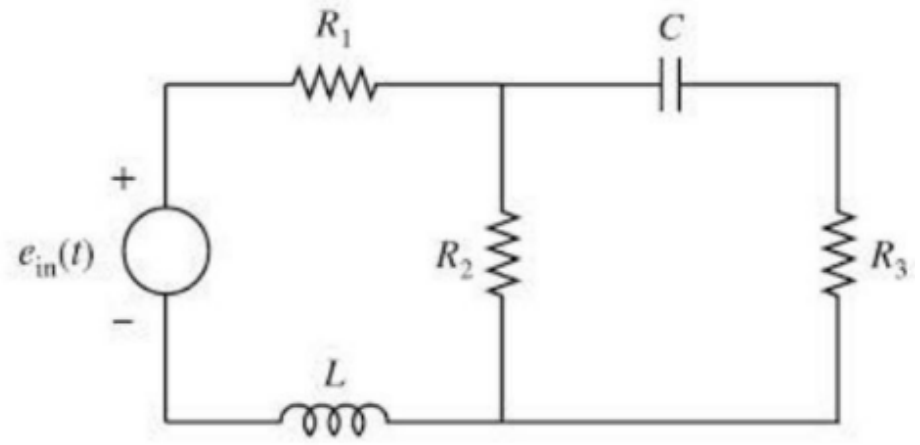
\includegraphics[scale = 0.7]{images/circuit.png}
\label{filtro1}
\caption{Circuito elétrico RLC}
\end{figure}

\subsection{Modelo Matemático do sistema}
Devemos encontrar o modelo matemático do sistema.

\subsection{Resposta Dinâmica do Sistema - Simulink}
Com base no modelo matemático, devemos encontrar a resposta do sistema (tensão e corrente nos capacitores) utilizando o Simulink, com os parâmetros a seguir:\\

$e_{in} = 12V$ \\
$R_1 = 2\Omega$ \\
$R_2 = 3 \Omega$ \\
$R_3 = 6 \Omega$ \\
$C = 0.03 F$ \\
$L = 0.2 H$ \\
$Tempo \>\ de \>\ simulação = 1s$ \\ \\


\subsection{Resposta Dinâmica do Sistema - Simscape}
Encontramos a resposta do sistema usando Simscape, com os mesmos parâmetros do item anterior.

\subsection{Parâmetros do sistema com o MATLAB}
Criams um script no MATLAB para definição dos parâmetros do sistema e execução dos dois modelos (Simulink e Simscape).

\subsection{Gráficos da Resposta do Sistema}
Geramos os gráficos das respostas do sistema. 

\subsection{Comportamento do Sistema}


\subsection{Analisando a diferença de comportamento}


\newpage
% REFERENCIAS %%%%%%%%%%%%%%%%%%%%%%%%%%%%%%%%%%%%%%%%%%%%%%%%%%%%%%%%%%%%%%

\nocite{*}
\bibliography{src/bibliography}
    
\end{document}
\section{Referências Bibliográficas}



\end{document}